\chapter{A review of the literature}
\label{chap:lit-review}

\section{Fluid-elastic galloping}
\label{fluid-elastic galloping}

Fluid-elastic galloping is one of the common observable flow-induced vibration modes of a slender body. Because this phenomenon is most common in civil structures, such as buildings and iced-transmission lines. The term ``aeroelastic galloping" is commonly used as the body is driven by wind. However, this mechanism can occur on a slender body immersed in any Newtonian fluid, provided that the conditions to sustain the galloping mechanism are satisfied. This work is based on a general Newtonian flow, thus the term `` fluid-elastic galloping" is used throughout this thesis.
   

\subsection{Excitation of galloping}
\label{sec:exci-galloping}

\citet{Paidoussis2010} describe galloping as a ``velocity dependent and damping controlled" phenomenon. Therefore, in order for a body to gallop, an initial excitation has to be given to that body. While this excitation is mainly caused by the force created from vortex shedding, other fluid instabilities may contribute to this initial excitation.  When a bluff body moves along the transverse direction of the fluid flow, it generates a force along the transverse direction. This force, also known as the induced lift, is a result of the fluid flow and the motion of the body. When this body is attached to a flexible system (i.e. a system that can be modelled by a spring, mass and damper), the induced lift becomes the forcing of the system. Galloping is sustained  if the induced lift is periodic and in phase with the motion of the body.

\begin{figure}
\setlength{\unitlength}{\textwidth}

  \begin{picture}(1,0.23)(0,0.74)
    
  \put(0.2,0.76){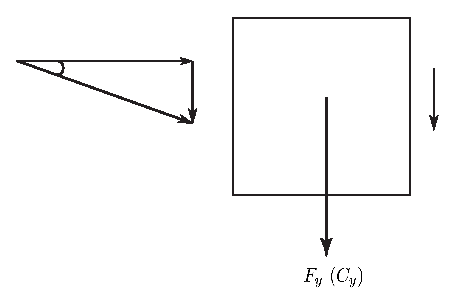
\includegraphics[width=0.5\unitlength]{../FnP/gnuplot/setup-1.eps}}         
      
      
   
 	\put(0.315,0.93){$U$}
 	\put(0.3,0.84){$U_i$}
    \put(0.42,0.88){$\dot{y}$}
    \put(0.28,0.895){ $\theta$}
    \put(0.7,0.87){\small $(+)$}
      	

 	
 	 

     

  \end{picture}

 \caption{Induced angle of attack on the square prism due to the resultant of free-stream velocity of the fluid and transverse velocity of the body.}
    \label{fig:setup_1}
\end{figure}

\begin{figure}[!h]
\setlength{\unitlength}{\textwidth}

  \begin{picture}(1,0.4)(0,0.74)
    
  \put(0.2,0.76){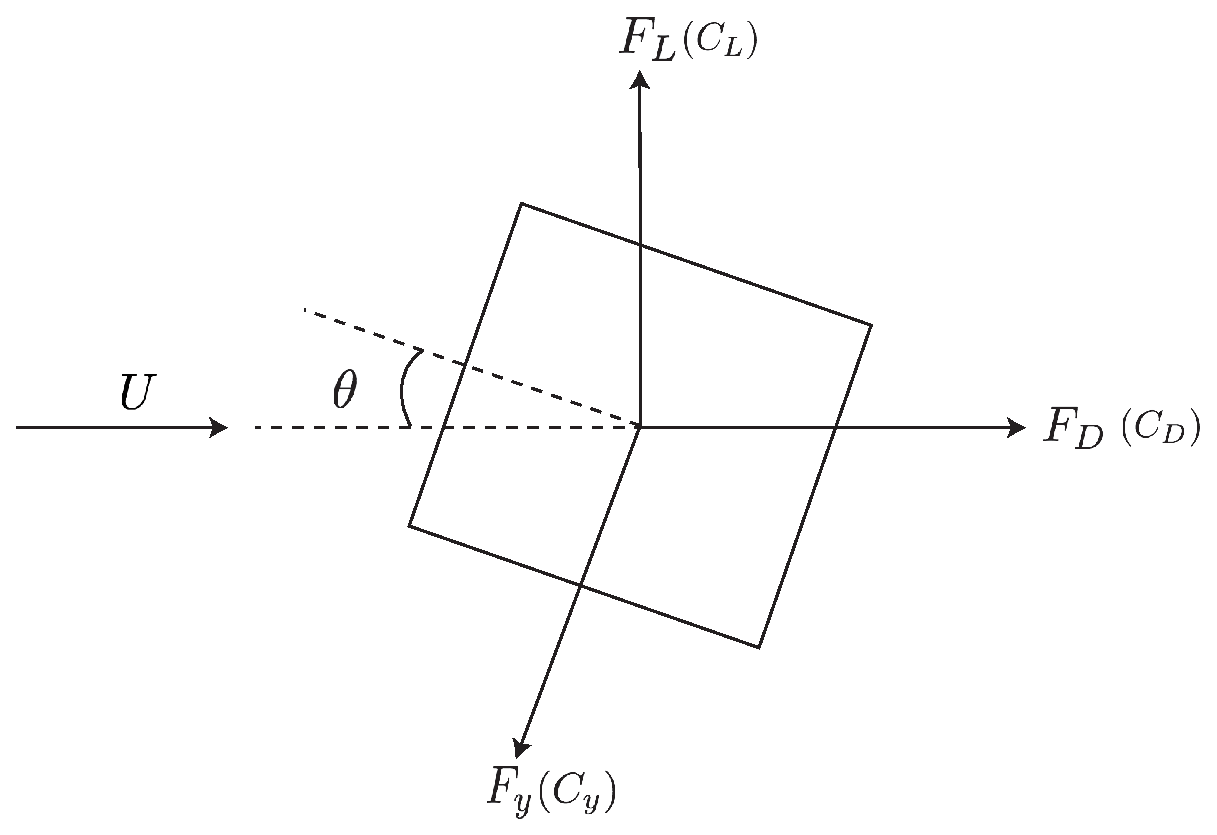
\includegraphics[width=0.5\unitlength]{./chapter-literature-revirw/fnp/f_y-illustration.eps}}         
      
      
   
% 	\put(0.315,0.93){$U$}
% 	\put(0.3,0.84){$U_i$}
%    \put(0.42,0.88){$\dot{y}$}
%    \put(0.28,0.895){ $\theta$}
%    \put(0.7,0.87){\small $(+)$}
      	

 	
 	 

     

  \end{picture}

 \caption{}
    \label{fig:f-y-sketch}
\end{figure}

A square cross section can be used as an example to further explain the galloping phenomenon. Figure \ref{fig:induced_lift_sketch}  illustrates the motion of the body at a given instant. The induced angle of attack is formed on the square cross section as a result of the free stream velocity vector $U$ and the transverse velocity vector of the body $\dot{y}$. An angle of attack implies that there will be a non-zero lift force on the body. Thus, a force is formed in phase with the velocity of the body. While illustated for the square, this mechanism can also be observed on any body that can have an angle of attack. The sign convention in this figure (and generally used in this scope of research) states that downward direction is positive.  

\subsection{Quasi-steady state theory}
\label{sec:QSS theory}


The vibrations caused in iced electric transmission lines was the key phenomenon which compelled researchers into studying fluid-elastic galloping. Some of the earlier work by \cite{Glauert1919} and \cite{DenHartog1956} lead to the pioneering study on galloping by \cite{Parkinson1964} which produced a mathematical model for a system under the influence of fluid-elastic galloping. A non-linear oscillator model was developed by Parkinson and Smith to predict the response of the system. Since then, this model has been widely used in almost all subsequent studies on galloping. Essentially, the model assumes the flow is quasi-steady. This means that the instantaneous induced lift force of the oscillating body is equal to that of the lift force generated by the same body when static at the same induced angle of attack. For the quasi-steady assumption to be valid, the conditions below have to be satisfied.

\begin{itemize}
 \item The velocity of the body does not change rapidly
 \item There is no interaction between vortex shedding and galloping
\end{itemize}

Both of these conditions imply that the vortex shedding frequency must be much higher than the galloping frequency.

The oscillator equation was solved using the Krylov and Bogoliubov method \citep{Parkinson1964}. The results obtained from experiments, carried out at $\reynoldsnumber=2200$ and a mass ratio (\mstar) around 1164 had a good agreement with the theoretical data which is shown in figure \ref{fig:parkinson_paper_data}. The details of this quasi-steady model are provided in section \ref{sec:qss_model}.

\begin{figure}
	
  \setlength{\unitlength}{\textwidth}

        \begin{picture}(1,0.82)(0,0.4)

      % % % Parkinson Data 

      \put(0.05,0.39){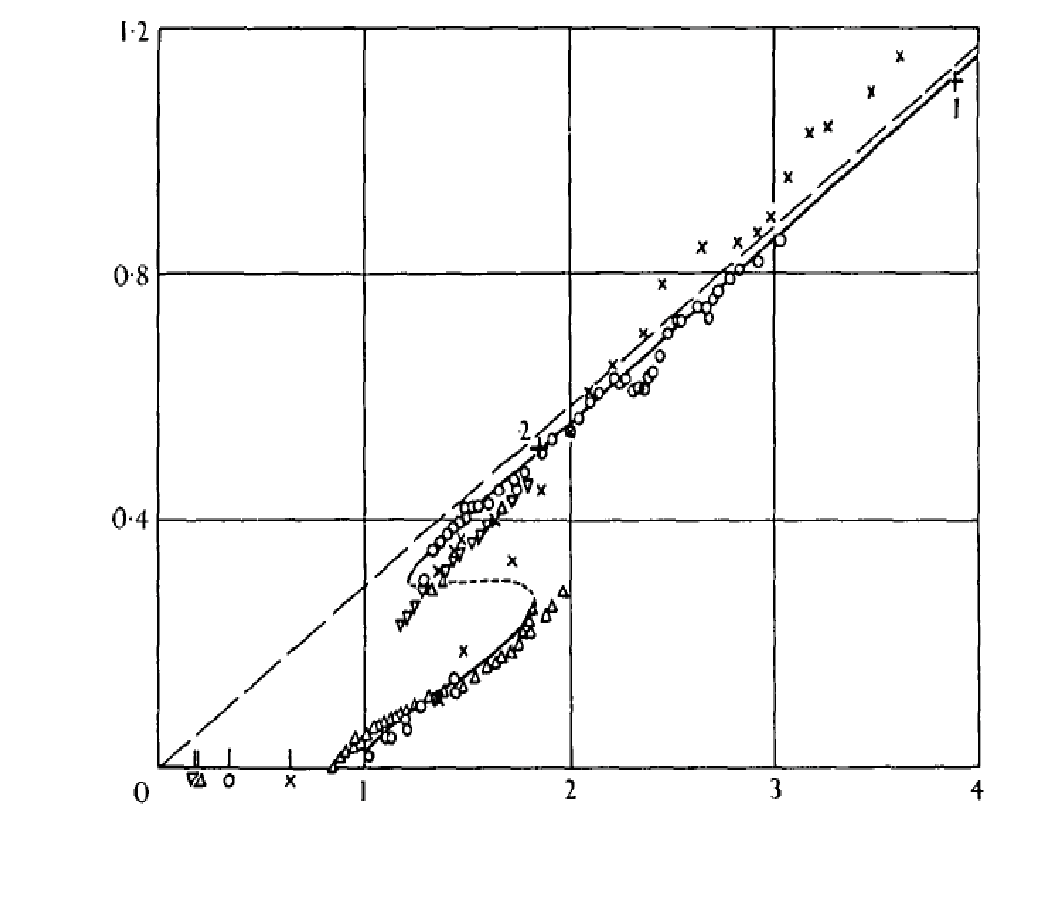
\includegraphics[width=0.9\unitlength]{./chapter-literature-revirw/fnp/parkinson_data.eps}}
      
%       \put(0.07,0.95){$\displaystyle\frac{V}{D}$}
%       \put(0.07,1.3){$\displaystyle\frac{A}{D}$}
       \put(0.05,0.8){\Large$\frac{nA}{2\beta}\bar{Y}_s$}
       \put(0.52,0.42){\Large$\frac{nA}{2\beta}U$}
       \
%\put(0.189,1.415){\small(a)}
%\put(0.189,1.07){\small(b)}
%\put(0.189,0.73){\small(c)}

%  


    \end{picture}

  \caption{``Collapsed amplitude-velocity characteristic. Theory: \solidrule \ stable limit cycle, \dashedrule unstable limit cycle. Experiment $\times \ \beta = .00107$, $\circ \ \beta =.00196$,\ $\vartriangle \beta=.00364$,$\triangledown \ \beta = .00372$,\ $+1 \ \beta=.0012$,\ $+2 \ \beta=.0032$ Reynolds numbers $4,000-20,000$ ". Figure extracted from \cite{Parkinson1964}. $\frac{nA}{2\beta}\bar{Y}_s$ is the dimensionless displacement amplitude parameter and $\frac{nA}{2\beta}U$ is the reduced velocity.$\beta$ is the damping ratio and $n=\frac{1}{\mstar}$. The experimental data shows a good agreement with the theoretical model.}
    \label{fig:parkinson_paper_data}
\end{figure}

 %vspace{10cm}


Figure \ref{fig:parkinson_paper_data} shows the comparison of data between the mathematical model and the experimental data of \citep{Parkinson1964}. The data shows a good agreement between the model and the experiments.  

\subsubsection*{Quasi-steady state oscillator model}
\label{sec:qss_model}

A simple transversely oscillating system with external driving force could be modelled with a spring, mass, damper system which can be expressed as,   

\begin{equation}
\label{equationofmotion_1}
m\ddot{y}+c\dot{y}+ky=\mathcal{Q},
\end{equation}

where the forcing term $\mathcal{Q}$ is the external force which drives the system.

Thus, the quasi-steady equation of motion of a transversely oscillating body under galloping, with linear springs and damping could be expressed by replacing the forcing term with the induced force (explained in section \ref{sec:QSS theory}) and could be expressed as,  

\begin{equation}
\label{equationofmotion}
m\ddot{y}+c\dot{y}+ky=F_y,
\end{equation}
where the forcing term $F_y$ is given by
\begin{equation}
\label{lift equation}
F_y=\frac{1}{2}\rho U^2\mathcal{A}C_y.
\end{equation}

As explained in section \ref{sec:QSS theory}, the quasi-steady assumption uses the stationary $C_y$ data for varying angles of attack as inputs to the oscillator equation. \citet{Parkinson1964} used a $7^{th}$ order odd curve fit to interpolate the stationary $C_y$ data as a function of the angle of attack. The order of the polynomial can be chosen arbitrarily depending on the study. For example \citet{Barrero-Gil2009,Barrero-Gil2010a} used a $3^{rd}$ order polynomial in order to simplify the analytical model. However, \citet{Ng2005} pointed out that a $7^{th}$ order polynomial is sufficient as higher order polynomials do not provide a significantly better result. Using a $7^{th}$ order polynomial sees the lift coefficient as a function of the angle of attack $\theta$ modelled as

\begin{equation}
\label{cy ploynomial}
C_y(\theta)=a_1\left(\frac{\dot{y}}{U}\right)-a_3\left(\frac{\dot{y}}{U}\right)^3+a_5\left(\frac{\dot{y}}{U}\right)^5-a_7\left(\frac{\dot{y}}{U}\right)^7.
\end{equation}

By substituting this forcing function into the oscillator equation (Eq:\ref{equationofmotion}) the quasi-steady state (QSS) model can be obtained as

\begin{equation}
\label{final_equation_motion}
m\ddot{y}{+}c\dot{y}{+}ky{=}\frac{1}{2}\rho U^2 \mathcal {A} \Bigg(a_1\left(\frac{\dot{y}}{U}\right){-}a_3\left(\frac{\dot{y}}{U}\right)^3{+}a_5\left(\frac{\dot{y}}{U}\right)^5{-}a_7\left(\frac{\dot{y}}{U}\right)^7 \Bigg).
\end{equation}

As the current study is focused on the low \reynoldsnumber\ region, it is a known fact that the vortex shedding will be well-correlated along the span and therefore provide a significant forcing. \citet{Joly2012} introduced an additional sinusoidal forcing function to the model in order to integrate the forcing by vortex shedding. By the addition of this forcing \citet{Joly2012} managed to obtain accurate predictions of the displacement amplitude even at low mass ratios, where the galloping is significantly suppressed by the vortex shedding to the point that it is no longer detectable. However, the strength or the amplitude of this sinusoidal forcing needed to be tuned in an \emph{ad hoc} manner, and the relationship between this forcing and the other system parameters was not clear. Thus in the current study this forcing is not used.


\subsubsection*{Presence of hysteresis}


\cite{Parkinson1964} observed a hysteresis region when the displacement amplitude was plotted as a function of the reduced velocity. Essentially two amplitudes were observed for the same reduced velocity depending on the initial condition. This fact is quite vital for energy harvesting as two values of energy levels can present for the same reduced velocity. Thus, have to be careful in considering the initial conditions of the system to gain a higher power output.  

Although hysteresis was observed in the amplitude data of \cite{Parkinson1964}, the studies carried out by \citet{Barrero-Gil2009} and \citet{Joly2012} at much lower Reynolds numbers ($159\leq \reynoldsnumber\leq 200$), did not show any hysteresis. \citet{Luo2003} concluded that hysteresis was present due to the presence of an inflection point in the $C_y$ curve which was only observed at high Reynolds numbers (\citet{Parkinson1964} data) and was not present at lower Reynolds numbers. It was further explained by \citet{Luo2003} the cause of this inflection point which was the intermittent reattachment of the shear layer at certain angles at occurred at high Reynolds numbers.   
 
\begin{figure}
	
  \setlength{\unitlength}{\textwidth}

  \begin{picture}(1,0.9)(0,0.75)

      % % % Parkinson Data 

      \put(-0.15,0.2){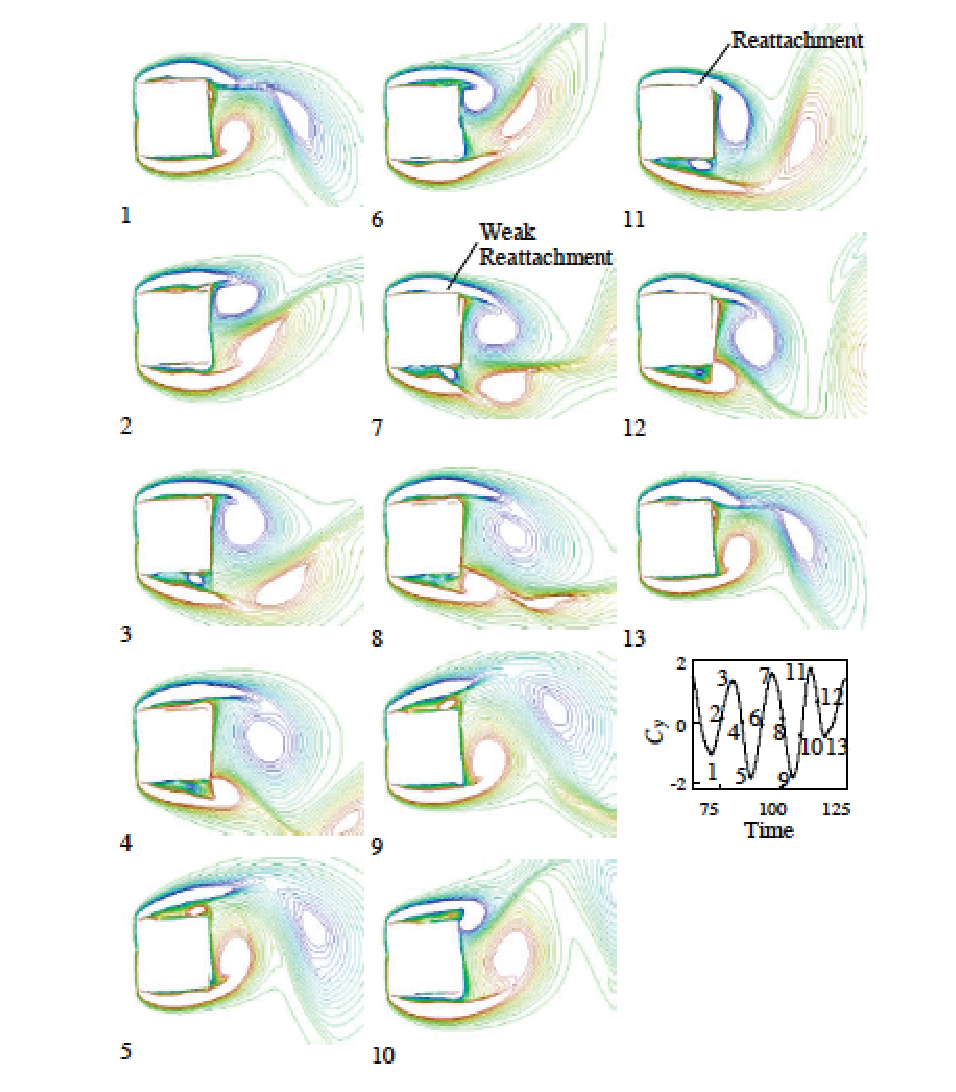
\includegraphics[width=1.3\unitlength]{./chapter-literature-revirw/fnp/luo-re-attachment.eps}}
      
%       \put(0.07,0.95){$\displaystyle\frac{V}{D}$}
%       \put(0.07,1.3){$\displaystyle\frac{A}{D}$}
      
%\put(0.189,1.415){\small(a)}
%\put(0.189,1.07){\small(b)}
%\put(0.189,0.73){\small(c)}

%  


    \end{picture}

  \caption{\label{fig:lit-review-luo-reattachment-1}Vorticity contours of \cy\ and the corresponding time for $\reynoldsnumber=1000$, $\theta=2^{\circ}$ extracted from \citet{Luo2003}. The intermittent shear level is visible in points 7 and 11}
\end{figure}


 %vspace{10cm}


Figure \ref{fig:lit-review-luo-reattachment} shows the vorticity contours of a square cross section obtained at various points of the vortex shedding cycle, at $\reynoldsnumber=1000$, $\theta=2^{\circ}$ obtained from \citet{Luo2003}using the  diffusion-vortex method and vortex-in-cell method. The points 7 and 11 show the intermittent shear layer reattachment which causes the hysteresis in the \cy\ vs. $\theta$ curve at high Reynolds numbers.

\vspace{20mm}   

\subsection{Induced force and the shear layers}
\label{subsec:c_y and shear layers}

 The quasi-steady model has already been validated and re-validated by many studies \citep{Parkinson1964,Barrero-Gil2009,Luo2003} and proven to model galloping. Since this model essentially assumes that the system is quasi-steady, the mean flow-field data of static body simulations at various angles of incidence can be used to analyse the behaviour of the instantaneous flow field of a galloping system at the same instantaneous induced angle. 
 
 
\begin{figure}[h]
\setlength{\unitlength}{\textwidth}

  \begin{picture}(1,0.46)(0,0.75)
    
  \put(0.2,0.76){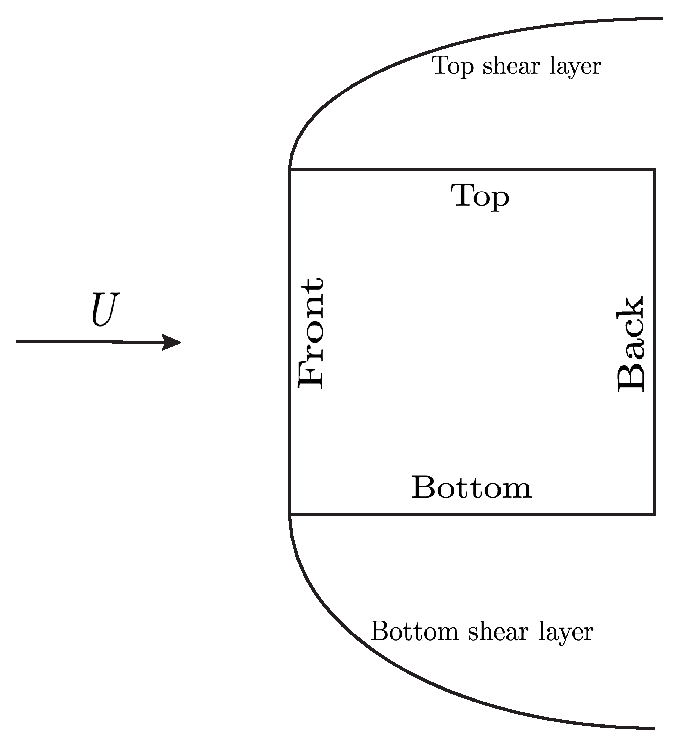
\includegraphics[width=0.4\unitlength]{./chapter-literature-revirw/fnp/shear-layer-sketch.eps}}         
      
      
   
 
 	
 	 

     

  \end{picture}

 \caption{Illustration of the top and bottom shear layers.}
    \label{fig:shear-layer-sketch}
\end{figure}

\begin{figure}[t!]

  \setlength{\unitlength}{\textwidth}

  \begin{picture}(1,0.35)(0,0.725)

    \put(-0.01,0.76){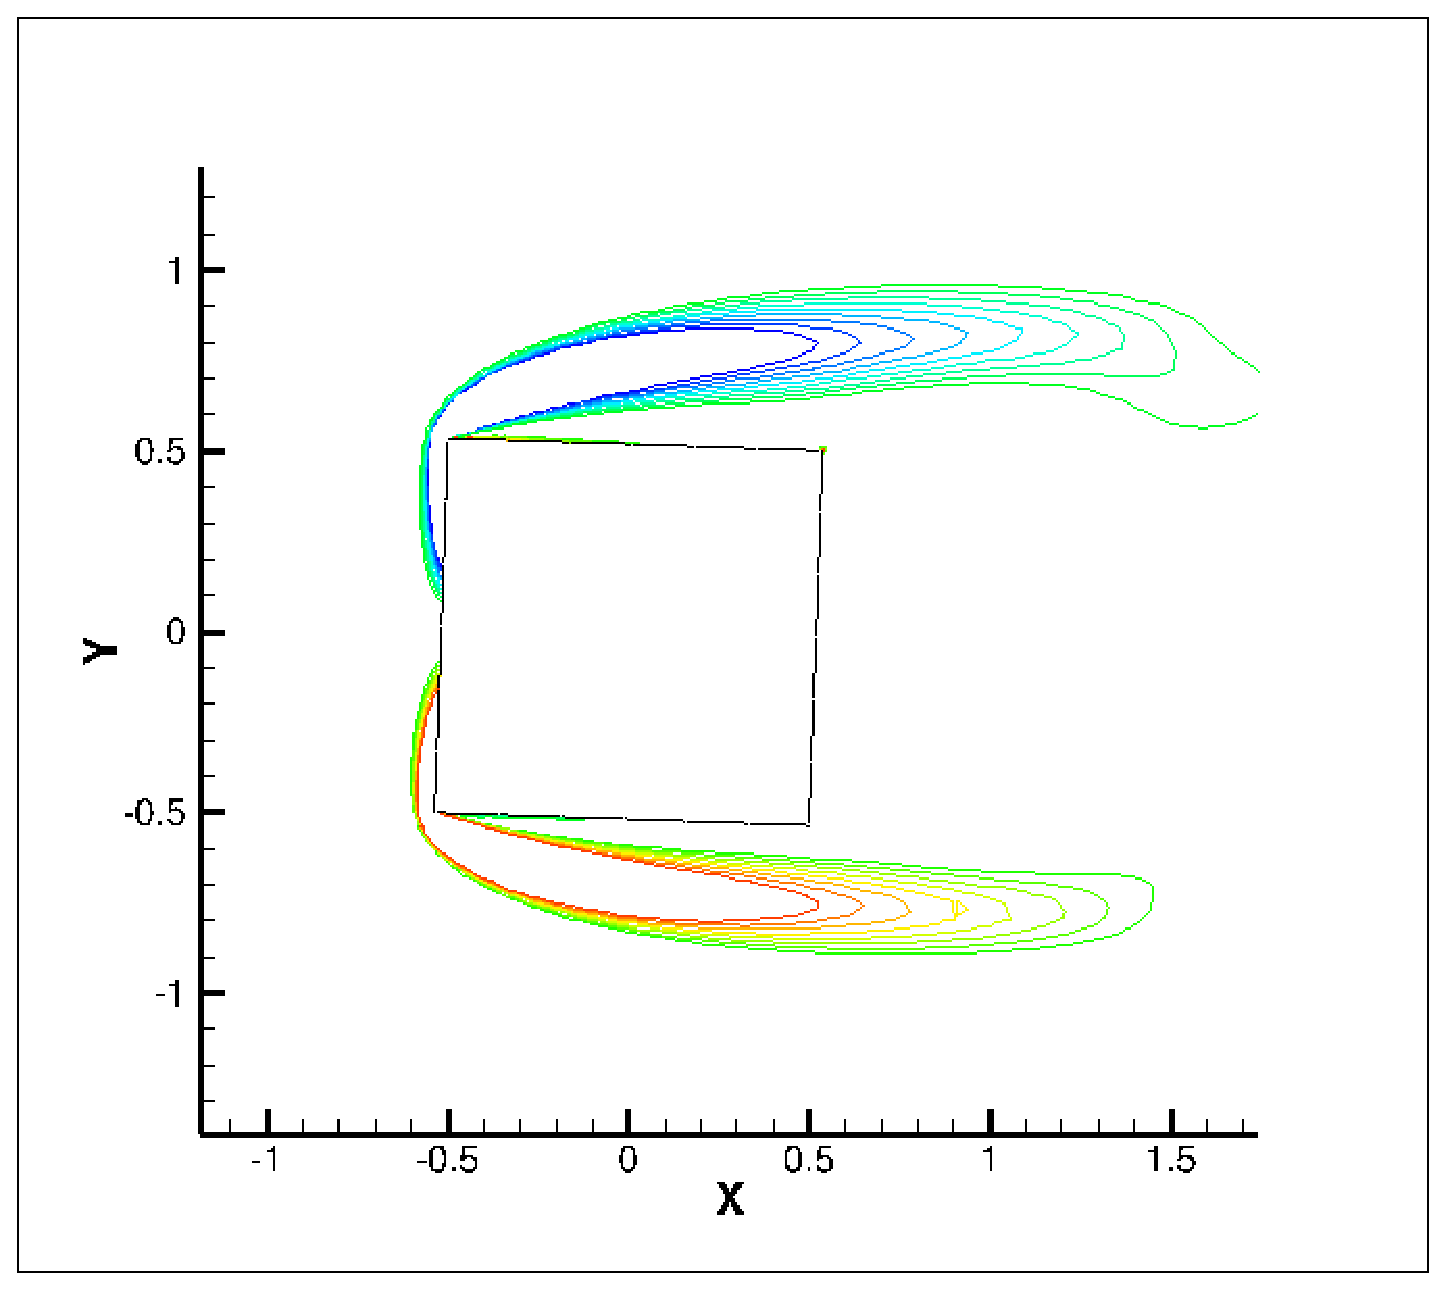
\includegraphics[width=0.33\unitlength]{./chapter-literature-revirw/fnp/square-2.eps}}
    \put(0.335,0.76){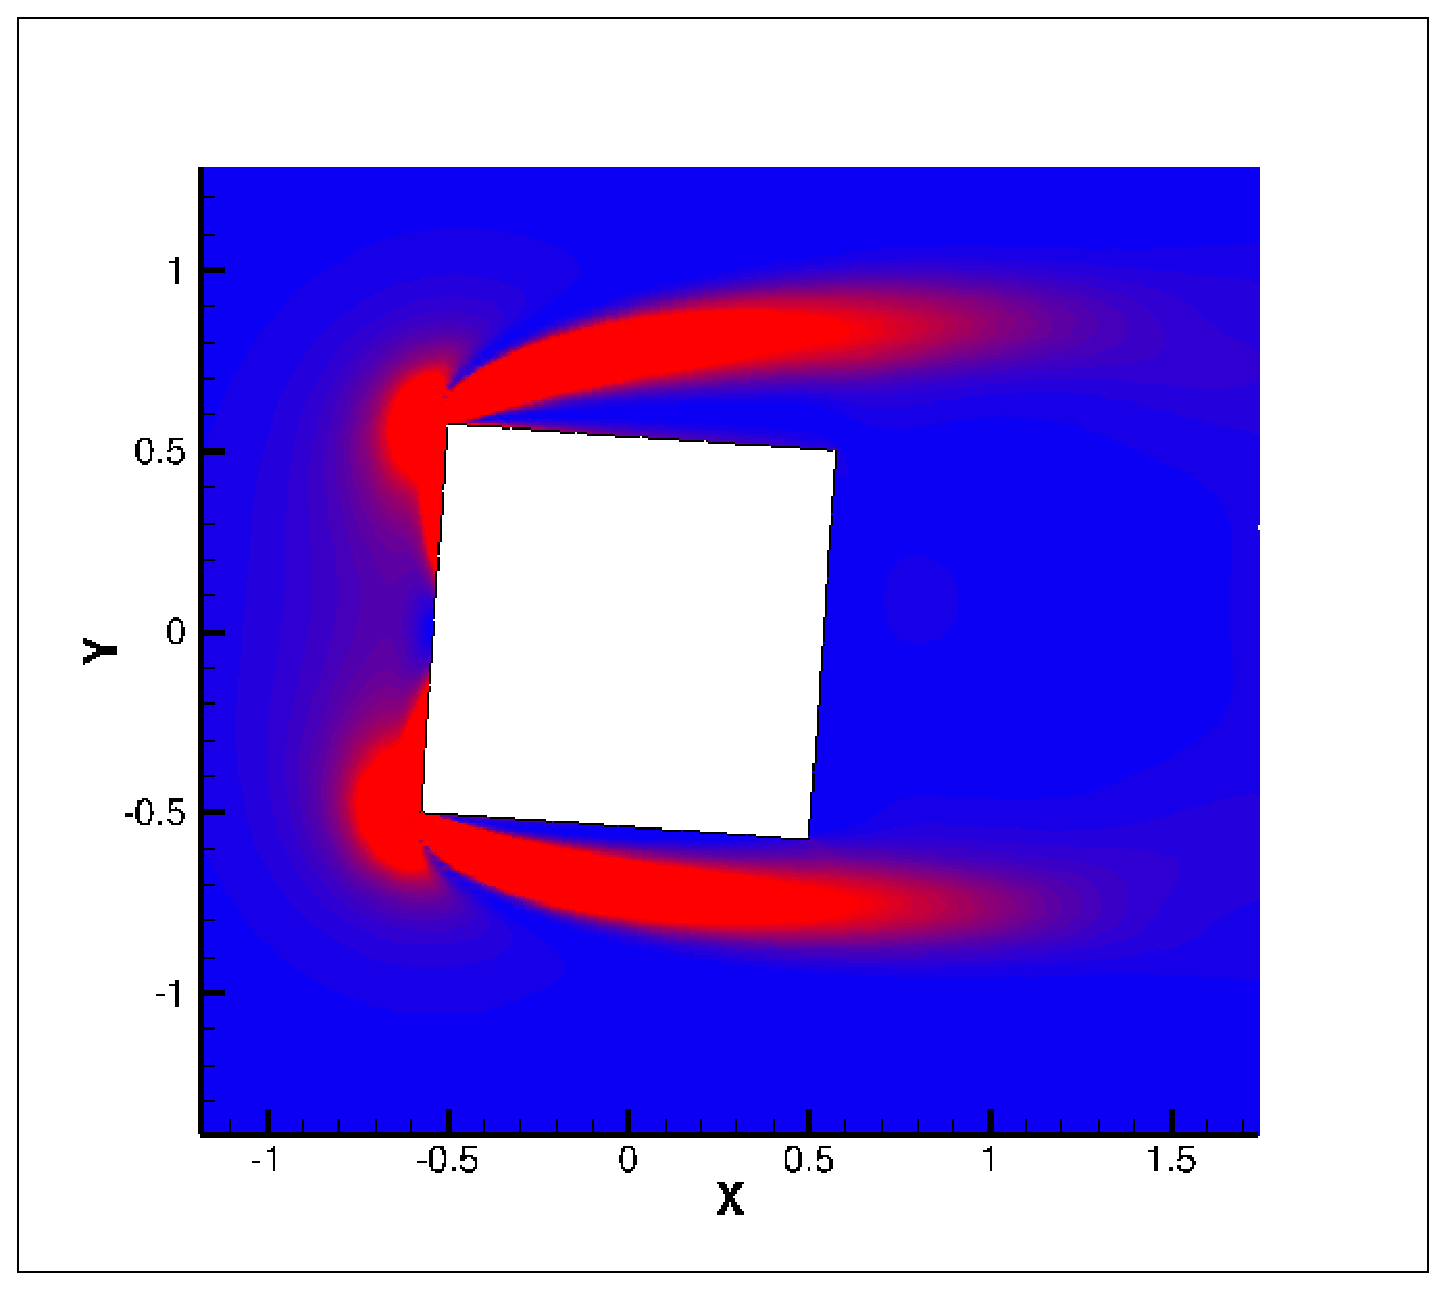
\includegraphics[width=0.33\unitlength]{./chapter-literature-revirw/fnp/square-4.eps}}
    \put(0.68,0.76){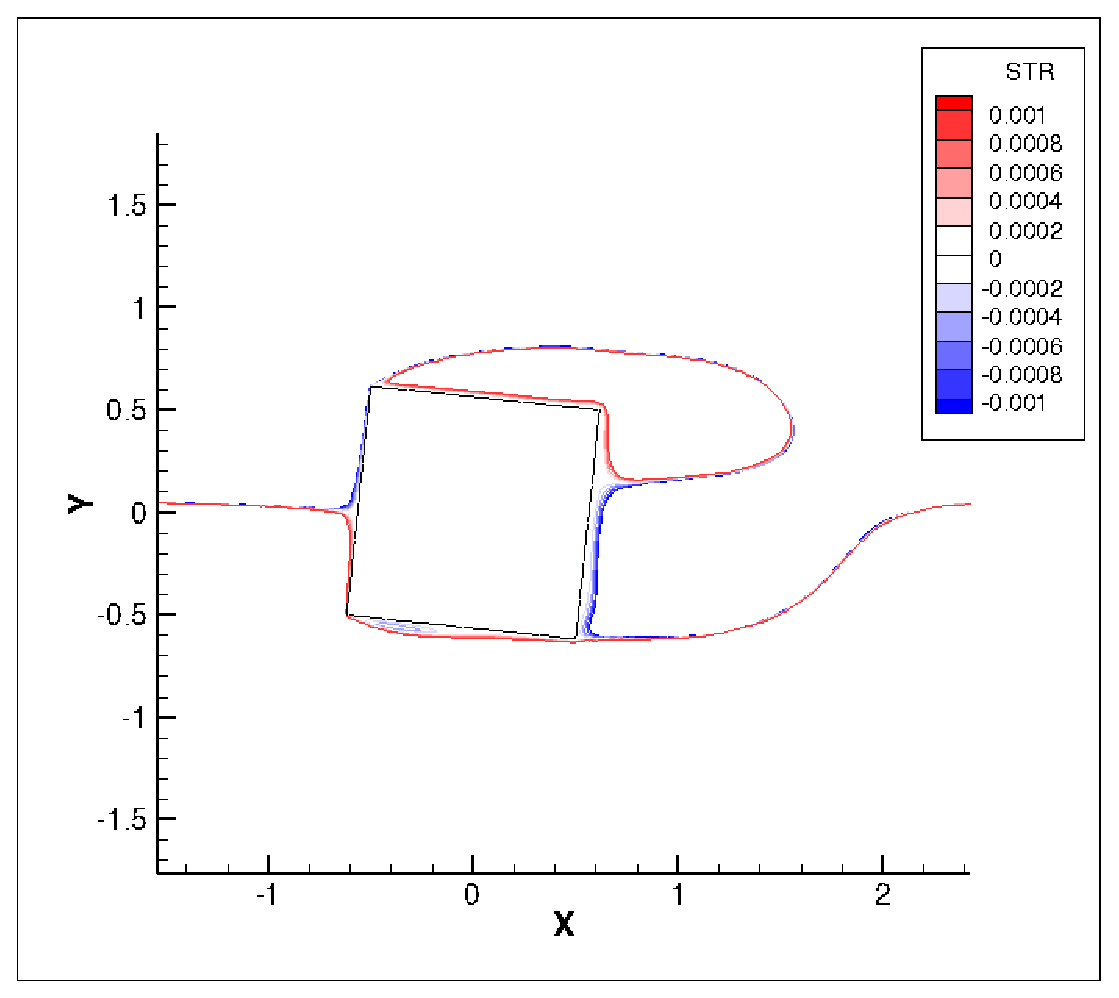
\includegraphics[width=0.33\unitlength]{.//chapter-literature-revirw/fnp/square-6.eps}}

   
    
    \put(0.0,0.735){(a)}    
    \put(0.34,0.735){(b)}
    \put(0.685,0.735){(c)}
  
  \end{picture}

  \caption{Stream functions of time averaged flow field on a stationary square section at $\reynoldsnumber=200$ at different incidence angles. (a) $2^{\circ}$ ($C_{y}$ increases),(b) $4^{\circ}$ ($C_{y}$ peaks) and (c) $2^{\circ}$ ($C_{y}$ decreases). The bottom shear layer comes closer to the bottom wall and reattaches as the angle of incidence increases.}
  \label{fig:shear_layers}
\end{figure}







\citet{Paidoussis2010,Parkinson1964,Barrero-Gil2010a} and many other published studies state that a system which sustains galloping should satisfy the condition that $\partial C_y/\partial \theta>0$, i.e, an upward motion from the equilibrium position should induce an upward lift force. The mean induced lift (\cy) occurs due to the unbalanced pressure distribution on the top and bottom sides of the afterbody of the cross section (refer figure \ref{fig:shear-layer-sketch}) when a small transverse velocity is given \citep{Parkinson1989}. This pressure difference of the afterbody is a result of the relative proximity of the top and bottom shear layers (illustrated in figure \ref{fig:shear-layer-sketch}) to the respective sides of the body. 

Contour plots of the shear strain rate magnitude, which is directly proportional to shear stress, for a static square cross section at various incidence angles shown in figure \ref{fig:shear_layers} clearly shows the behaviour of the shear layers at either sides of the body. Data are presented for three key incidence angles $2^{\circ}, 4^{\circ} \text{and}\ 6^{\circ}$ In comparison with figure \ref{fig:lift_curves} these points can be identified as being in regions where \cy\ initially increases, \cy\ is maximum and \cy\ decreases .Note that these data and plots are obtained from the current study for the purpose of providing a better illustration.

As the angle of incidence ($\theta$) increases clockwise from $2^{\circ}-6^{\circ}$, it can be clearly observed in figure \ref{fig:shear_layers} that the bottom shear layer comes closer to the bottom wall of the body compared to the top shear layer. The shear layer nearer to the body creates higher suction compared to the shear layer at the opposite side, as the higher velocity in the shear layer implies a lower pressure, from a simple Bernoulli-type argument. This pressure imbalance between the top and bottom sides of the body creates a downward force which with the sign convention introduced in figure \ref{fig:induced_lift_sketch} is positive. As the angle is further increased to $\theta=4^{\circ}$, the bottom shear layer comes even closer and therefore the pressure difference becomes greater leading to a higher $C_{y}$. The induced lift force \cy, becomes maximum when the shear layer near to the wall just reattaches at the trailing edge. As $\theta$ is further increased at  $\theta=4^{\circ}$ (figure \ref{fig:shear_layers} (b)), the recirculation region formed by the reattachment of the bottom shear layer shrinks in size resulting in a reduction of the velocity near the wall, and therefore an increase in pressure. This implies a reduction of the pressure imbalance between the top and bottom surface leading to the reduction in $C_{y}$. This theory has been discussed in \citet{Parkinson1989}. The variation of \cy\ vs $\theta$ is presented in figure \ref{fig:lift_curves}. As the body is connected to an oscillatory system (discussed in section \ref{sec:exci-galloping}), this shear layer behaviour also harmonizes with the cyclic behaviour of the system providing the driving force to the system so that the motion of galloping is sustained.

\subsection{Governing parameters of galloping}

From the published literature, it is observed from the earlier works such as \citet{Parkinson1961,Luo1994} to recent studies such as \citet{Luo2003,Barrero-Gil2010a,Joly2012} that classical VIV parameters have been incorporated to describe galloping. These parameters are the reduced velocity \ustar\ which is the velocity of the flow normalised by the natural frequency of the system and $\zeta$ which is the damping ratio based on the linear system in a vacuum. Both of these parameters consists of a frequency component. As VIV is a resonant type of phenomenon these parameters are suitable for VIV. However, as galloping is not a resonance-type phenomenon driven by the natural frequency, but a velocity driven phenomenon, these normalisations might not be suitable for galloping. This could be clearly observed in \citet{Barrero-Gil2010a}. In this study, which is focused on energy harvesting, the power curves presented using these current parameters does not provide a good collapse. Therefore, it is necessary to formulate new parameters which effectively describe galloping particularly the energy transfer between the fluid and the body as it is the focus of this study.     


\subsection{Frequency response}
 
 It is clear that the cyclic motion of the shear layer will harmonize with the mechanical system. Therefore, the frequency response should be close to the natural frequency of the system $\omega_{n}$ \citep{Paidoussis2010}. This is significantly different from the VIV mechanism, where the primary frequency comes from the periodic forcing of the vortex shedding. Hence, in the QSS model the natural frequency of the system can be identified as the frequency of oscillation. However, it should be  noted that this is valid on the regimes where the conditions discussed in section \ref{sec:QSS theory} are satisfied. 
 
 The experimental studies carried by \citet{bouclin:77} concluded at high reduced velocities with large inertia (where the natural frequency is very low), the motion of the body controls the frequency of the system rather than the vortex shedding. The structural damping has no effect provided that it is small. This study also concluded that as the inertia and the reduced velocity gets lower, there is some interaction between vortex shedding and galloping. When this occurs the frequency is mainly governed by the vortex shedding. 
 
 \subsection{Fluid mechanics governing the galloping response}
 \label{subsec:fluid_mechanics_of_galloping}
 
 As discussed in subsection \ref{subsec:c_y and shear layers} the driving force of a galloping system is the asymmetrical placement of the shear layers at either sides of the body. As a consequence, it is clear that a significant afterbody is needed for the shear layer interaction to sustain galloping. \citet{Parkinson1974,Parkinson1989} and \citet{Bearman1987} have discussed well the importance of the length and the shape of the body for galloping in their reviews. It is also highlighted in \citet{Parkinson1974} that the most important physical parameters for galloping are the size relative to the characteristic height and the shape of the afterbody. Manipulating the shape of the afterbody and thereby manipulating the shear layer interactions with the body, gives the ability to control the galloping response.
 
\citet{Blevins1990} provided a good comparison of the shapes which are prone to galloping based on the work by \citet{Parkinson1961}, \citet{Nakamura1975a} and \citet{Nakamura1977}. The reproduction of Blevins's data can be found in \citet{Paidoussis2010} and presented in figure \ref{fig:par_diff_cross_sec}. Here the induced angle is represented by $\alpha$ and the transverse force force coefficient is represented by $C_{fy}$. In order for galloping to sustain, the direction of both of these quantities should be same this thus have to satisfy the condition of 

\begin{equation}
\frac{\partial C_{fy}}{\partial \alpha } >0
\end{equation}  
    
 \begin{figure}
	
  \setlength{\unitlength}{\textwidth}

\fbox{
        \begin{picture}(1,1.2)(0,0.5)

      % % % Parkinson Data 

      \put(0.05,0.52){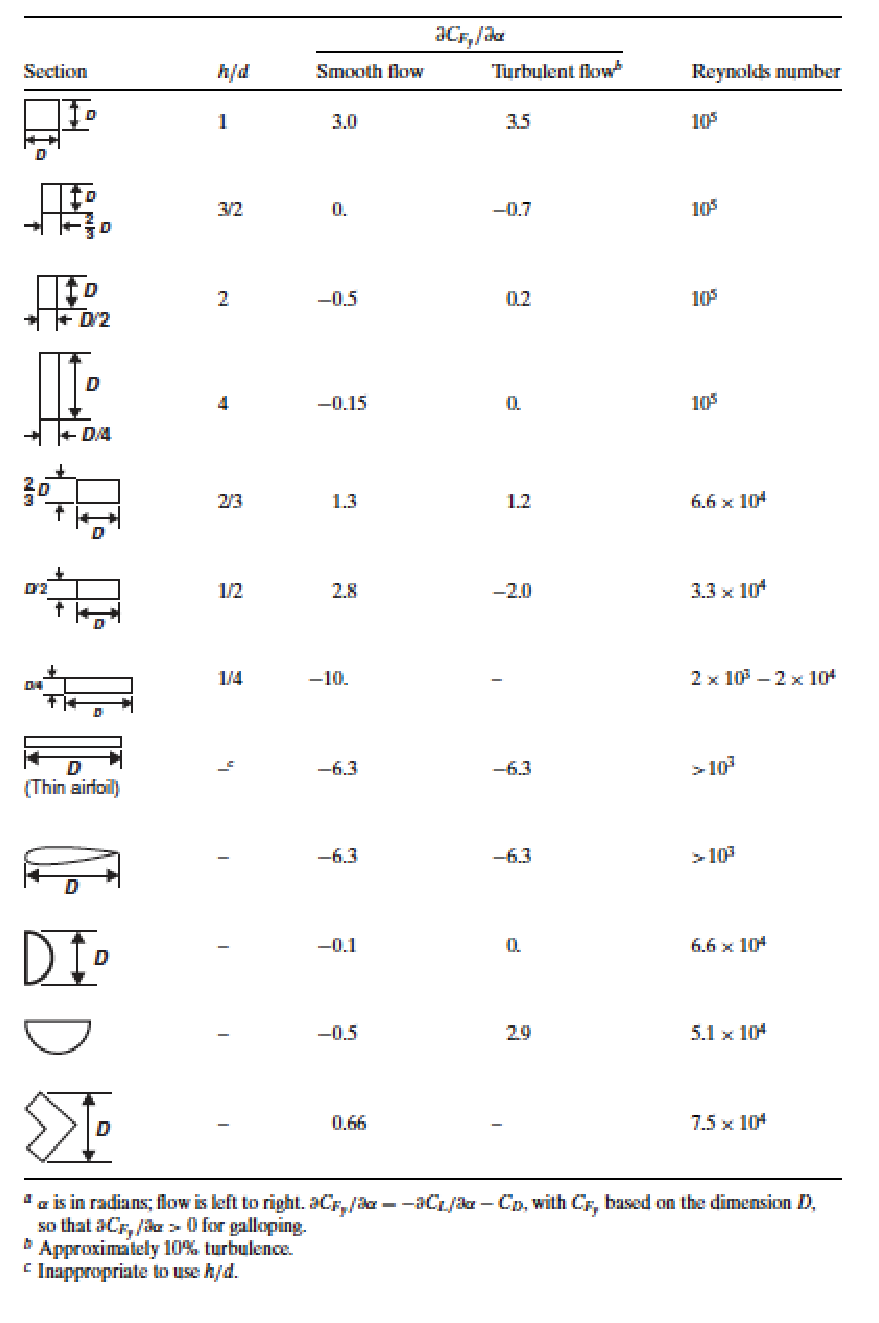
\includegraphics[width=0.75\unitlength]{./chapter-literature-revirw/fnp/per_cross_sec.eps}}
        


    \end{picture}
}
  \caption{ ``The transverse force coefficient for various sections in steady smooth or turbulent flow (after \citet{Blevins1990})" obtained from \citet{Paidoussis2010}. Here the induced angle is represented by $\alpha$ and the transverse force force coefficient is represented by $C_{fy}$. In order for galloping to sustain, the direction of both of these quantities should be same and thus have to satisfy the condition of $\frac{\partial C_{fy}}{\partial \alpha } >0$.}
    \label{fig:par_diff_cross_sec}
\end{figure}

 %vspace{10cm}

 
 
\citet{Naudascher1993}, \citet{Ruscheweyh1996}, \citet{Deniz1997} and \citet{Weaver2005} also provide data on different cross sectional shapes. \citet{Alonso2009} carried out wind tunnel tests on biconvex and rhomboidal cross sections. This study concluded that the galloping stability is dependent on the angle of attack. The aspect ratios where galloping is sustained in these cross sections were identified. Studies were further carried out by Alonso for elliptical cross sections \citep{Alonso2010} which concluded that galloping is Reynolds number dependent for elliptical cross sections. The study of triangular cross sections carried out by \citep{Alonso2005} isolated the angles of attack where galloping is sustained. The regions of stability for galloping at different angles of attack and the static force coefficients are presented in these studies with regards to the cross section involved. \citet{Luo1994} carried out an interesting study where the influence of the afterbody on galloping was investigated. The sides of a square section was chamfered gradually delaying the shear layer re-attachment, and two trapezoidal cross sections and one isosceles triangle was obtained. The \cy\ vs. $\theta$ plots revealed that the maximum value of \cy\ increased as the chamfering angle increased (i.e when the cross section was transformed from a square to a isosceles triangle). Anther interesting observation was that the incident angle where maximum \cy\ occurred increased as the chamfering angle increased. Delaying shear layer reattachment leads to higher \cy\ at higher induced angles which leads to higher induced velocities. This fact is beneficial for energy harvesting because as shown in equation \ref{eqn:power_alt} power is a function of both $F_{y}$ and the velocity of the body. \citep{Kluger2013} concluded that the best cross sectional shape for their "vibro-wind'' energy harvester was a trapezoidal cross section. However, this study has not revealed the underpinning fluid mechanics in detail such as the behaviour of the shear layers which makes an optimum cross section.

While many of these previous studies have investigated the influence of different body shapes on the galloping response, very few have systematically varied the shape of the body with the aim of deliberately amplifying the galloping. If galloping is to be used as an energy harvesting mechanism, finding an optimum body shape which produce large transverse velocities is desirable.


\subsection{Galloping as a mechanism of energy harvesting}

The focus of fluid-elastic galloping research in the past was on understanding and developing methods to suppress it, due to the adverse effects on civil structures. However, recently the focus of research has been redirected to develop mechanisms to excite galloping rather than suppressing it. This is due to the recent demand for alternative energy sources with minimal environmental impact. Thus, this demand for alternate energy has lead researchers to develop ways of extracting useful energy from flow induced vibrations.

Bernitsas and his group in the University of Michigan have made significant progress on using VIV as potential candidate for energy extraction. \cite{Bernitsas2008a-concept} introduced the concept of using VIV as a mode of energy extraction. The group have developed a device called VIVACE converter based on this concept. The work has been further expanded to focus on various aspects (such as Reynolds number effects, damping effects etc.) in \citet{Bernitsas2009,Raghavan2009,Raghavan2010a,Lee2011a}. This group has studied extensively on the effect of the mechanical parameters, the Reynolds number effects and the bottom boundary conditions of the VIVACE converter, in order to obtain efficient energy output using VIV as an energy harvesting mechanism. 

In contrast, the research carried out investigating the possibility of energy harvesting using fluid-elastic galloping is quite limited. \citet{Barrero-Gil2010a} conducted the pioneering study on energy harvesting using fluid-elastic galloping. The key consideration investigated in this study was that unlike VIV fluid-elastic galloping is not dependent on a synchronisation or a ``lock-in" mechanism. Therefore, it could operate on a wide spectrum of frequencies giving fluid-elastic galloping an advantage over VIV as a mechanism of energy harvesting. The study incorporated the QSS model where the Krylov and Bogoliubov method was used to solve the equation. This study used a $3^{rd}$ order polynomial rather than a $7^{th}$ order polynomial for simplification purposes which would have lead to less accurate quantitative results. However, This initial work showed that galloping could indeed used as a candidate for energy harvesting .\citet{vicente-Ludlam2014} showed that there is a link between the optimal electrical load resistance and the flow speed. This study was built on \citet{Barrero-Gil2010a} taking the QSS model as the mode of data acquisition. Similar to \citet{Barrero-Gil2010a} this study also incorporated a low order $3^{rd}$ order polynomial for the QSS model which again restricted the quantitative accuracy of the results. Since the work was mainly qualitative, it was identified that the understanding is primary and therefore step-by-step research has to be conducted in order to properly understand the link between energy transfer in the galloping mechanism and a experimental prototype should be developed to test the engineering performance. 

\citet{Kluger2013} from Cornell university have produced a prototype called "Vibro-wind" energy harvester which essentially uses the galloping mechanism. The mechanism used here differ slightly from the traditional transversely body where the oscillating body is connected with a cantilevered beam. Thus, there is both translational and rotational motion in the system. It was concluded that the amplitude of the galloping oscillator which couples the rational motion with the translational motion was always less that the amplitude of a body under a pure translational motion. As the present study is focused on theoretical aspects of the energy transfer, motion of the body is kept purely translational.   


\subsection{Review summary and statement of objectives}

 It is clear that more investigations should be carried out on energy transfer of a galloping system, particularly to develop efficient energy harvesting systems. More fundamental research is needed to explore the underpinning effects of mechanical and fluid dynamic parameters influencing the energy transfer of a galloping system to fill the gaps of the existing knowledge base. Thus, the objectives of the current research, spread over two phases, are defined as follows.
 
 \subsection*{Phase 1: Understand the governing mechanical parameters of the system and isolate regions of parameter space where a good power transfer can be obtained}
 
 \citet{Paidoussis2010} describes galloping as a ``velocity dependent damping controlled phenomenon". Yet, so far the scaling parameters used in studies are the traditional VIV parameters which are the damping ratio $\zeta$ and the reduced velocity \ustar\ \citep{Barrero-Gil2010a} which has a embedded frequency component. Thus following objectives were defined for this phase 
 
 \begin{itemize}
\item Formulate a new set of scaling parameters based on the natural time-scales of the system.
\item Investigate the influence of these parameters on mean power transfer.
\item Isolate the regions where high power transfer can be obtained.
\item Investigate the relationship between these new scaling parameters and the frequency response of the system. 
 \end{itemize}
 
    
  \subsection*{Phase 2: Understand the fluid mechanics of the system and optimise and control these mechanics to obtain a higher power transfer}
  
  \citet{Luo1994} showed that inhibition of shear layer reattachment could lead to higher peak $F_{y}$ at higher induced angles and therefore higher transverse velocities. Thus, from equation \ref{eqn:power}, it can be hypothesised that a higher mean power can be obtained by inhibition of the shear layer reattachment. Hence, the following objectives were defined for phase 2. 
  
  \begin{itemize}
  	\item Obtain QSS power data by systematically delaying the shear layer and investigate the influence on power.
  	\item Identify the relationship between the flow structures and the mean power output through analysis of the flow-field.
  	\item Provide design considerations for a galloping energy extraction system based on passive control of the shear layers. 
  \end{itemize}
 
 
 The stated aims are addressed by the following sections. Objectives of phase 1 are addressed in chapter \ref{chap:pi_1_pi2}. A new set of scaling parameters namely the combined mass stiffness \massstiff\ and the combined mass damping \massdamp\ are formulated from the linearised QSS model. The power data of obtained from numerically solving the QSS model and direct numerical simulations are presented though the new parameters and compared against the classical VIV parameters. Furthermore, an expression for the frequency of the system is formulated in terms of \massstiff\ and \massdamp. The data obtained though this model are compared against data acquired though QSS model and DNS. 
 
 
 Chapter \ref{chap:cross-sections} addresses the objectives of phase 2, where the possibility of achieving higher power transfer though the inhibition of shear layer reattachment is investigated. The inhibition of the shear layer reattachment is achieved by altering the afterbody of the square cross section. The mean power data of these cross sections obtained using the QSS model and DNS are analysed and compared. Key regions of the \cy\ vs. $\theta$ curve which significantly influences the power transfer are analysed and compared. Through this comparison, design considerations for an efficient galloping energy harvesting system are discussed.        